%%%%
% Consiglio la visione dei seguenti tutorial:
% - https://www.youtube.com/watch?v=ihxSUsJB_14
% - https://www.youtube.com/watch?v=XTFWaV55uDo
%%%%
\documentclass[12pt,a4paper,openright,twoside]{book}
\usepackage[utf8]{inputenc}

%\newcommand{\thesislang}{italian} % decommentare in caso di tesi in italiano
\newcommand{\thesislang}{english} % commentare in caso di tesi in italiano
\usepackage{thesis-style}
% version
\newcommand{\versionmajor}{0}
\newcommand{\versionminor}{1}
\newcommand{\versionpatch}{2}
\newcommand{\version}{\versionmajor.\versionminor.\versionpatch}
\typeout{Document version: \version}

\begin{document}
	
\frontmatter

% ! TeX root = thesis-main.tex
\title{Title}
\author{Candidate Name Here}
\date{\today}

\newgeometry{margin=0.8in}
\begin{titlepage}
	\begin{center}
		% \vspace*{0.2cm}
		
		\large
		\textbf{ALMA MATER STUDIORUM -- UNIVERSITÀ DI BOLOGNA \\ CAMPUS DI CESENA}
		\\
		\noindent\hrulefill
		\vspace{0.4cm}
		
		\Large
		Scuola di Ingegneria e Architettura \\
		Corso di Laurea (Magistrale) in Ingegneria e Scienze Informatiche
		
		\Huge
		\vspace{4cm}
		\textbf{
			Fair-by-design matching algorithm
		}
		
		\large
		\vspace{1cm}
		Tesi di laurea in 
		\\
		\textsc{(Intelligent System Engineering)}
		
		\vspace{5.5cm}
		\begin{minipage}[t]{0.64\textwidth}
			\begin{flushleft}
				\textit{Relatore} 
				\\ 
				(\textbf{Prof.} $\mid$ \textbf{Dott.}) \textbf{Nome Cognome}
				\\
				\vspace{0.4cm}
				\textit{Correlatore} 
				\\
				(\textbf{Ing.})? \textbf{Dott.} \textbf{Nome Cognome}
			\end{flushleft}
		\end{minipage}
		\begin{minipage}[t]{0.34\textwidth}
			\begin{flushright}
				\textit{Candidato} 
				\\ 
				\textbf{Antonio Iannotta}
			\end{flushright}
		\end{minipage}\\
		
		\vfill
		\noindent\hrulefill
		\vspace{0.3cm}
		\Large
		
		%(N-Esima) Sessione di Laurea
		II Sessione di Laurea
		\\
		Anno Accademico 2022-2023
	\end{center}
\end{titlepage}
\restoregeometry


\begin{abstract}	
Artificial Intelligence (AI) has revolutionized many sectors, including matching, by providing automated solutions for resource, opportunity, or information associations. However, the widespread use of matching algorithms in AI can also lead to potential discrimination, amplifying existing inequalities in society. This thesis focuses on the development of fair-by-design algorithms for matching in the field of artificial intelligence to ensure ethical, transparent, and non-discriminatory association decisions.

Throughout the research, various fundamental aspects of matching in the context of AI and the associated ethical implications are examined. The main challenges related to discrimination, fairness, and transparency in the matching process are identified. Subsequently, the current approaches and methodologies available for developing fair-by-design algorithms are presented and analyzed.

The thesis proposes a novel approach to matching that integrates fairness and discrimination criteria within the algorithmic process. Different fairness and discrimination metrics are explored to assess the impact of matching algorithms on the distribution of opportunities and equitable treatment of different user categories.

The implementation of fair-by-design algorithms for matching is evaluated through a series of case studies, where the performance of the proposed algorithms is analyzed and compared to conventional solutions. The results demonstrate that fair-by-design algorithms can significantly reduce disparities and discrimination compared to traditional matching methods.

Finally, guidelines are proposed for developers and stakeholders interested in matching in the field of AI, aiming to promote the adoption of fair-by-design algorithms and encourage ethical and responsible use of artificial intelligence.
\end{abstract}

\begin{dedication} % this is optional
Optional. Max a few lines.
\end{dedication}

\begin{acknowledgements} % this is optional
Optional. Max 1 page.
\end{acknowledgements}

%----------------------------------------------------------------------------------------
\tableofcontents   
\listoffigures     % (optional) comment if empty
\lstlistoflistings % (optional) comment if empty
%----------------------------------------------------------------------------------------

\mainmatter

%----------------------------------------------------------------------------------------
\chapter{\introductionname}
\label{chap:introduction}
%----------------------------------------------------------------------------------------

Write introduction here.

%
\paragraph{Thesis Structure.} % Optional paragraph title
%

(This is optional an optional paragraph.)
%
Accordingly, the reminder of this thesis is structures as follows.
%
\Cref{chap:background} discusses (briefly describe the content of \cref{chap:background}).
%
Describe other chapters here in a similar way.
%
Finally, \Cref{chap:conclusions} concludes this thesis by summarising its main contribution.

%----------------------------------------------------------------------------------------
\chapter{State of the Art} % or Background
\label{chap:background}
%----------------------------------------------------------------------------------------

%Write background here.

%This section is likely to contain a lot of citations.
%
%For instance in \cite{AnzengruberSocInfo2013} the authors propose a novel means for tackling with the problem of preventing bad things from happening.

%----------------------------------------------------------------------------------------
\chapter{Design} % possible chapter for Projects
\label{chap:design}
%----------------------------------------------------------------------------------------

Write design here.

\begin{figure}
	\centering
	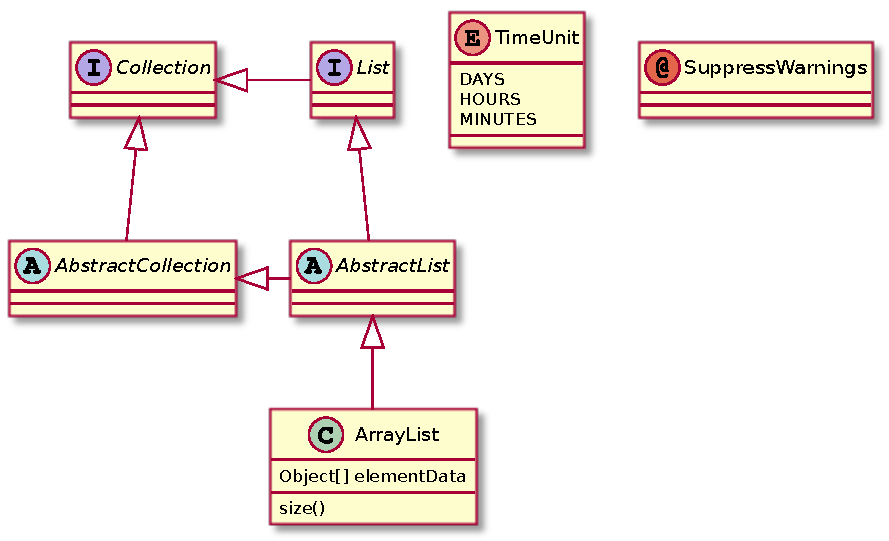
\includegraphics[width=0.5\linewidth]{figures/classes.pdf}
	\caption{A class diagram created with PlantUML}
	\label{fig:classes}
\end{figure}

You may want to reference images in your thesis.
%
In this case, you are encouraged to make them \emph{floating}, and reference them by means of labels.
%
For instance, in \Cref{fig:classes}, we describe a class diagram produced by means of \href{http://plantuml.com}{PlantUML}.

%----------------------------------------------------------------------------------------
\chapter{Implementation} % possible chapter for Projects
\label{chap:implementation}
%----------------------------------------------------------------------------------------

Write implementation here.

\lstinputlisting[
	float,
	language=Java,
	caption={My very first program in Java},
	label={lst:helloworld},
]{listings/HelloWorld.java}

You may need to reference listings in your thesis.
%
In this case, you are encouraged to make them \emph{floating}, and reference them by means of labels.
%
For instance, in \Cref{lst:helloworld}, we describe an hello world program in Java.

%----------------------------------------------------------------------------------------
\chapter{Validation} % possible chapter for Projects
\label{chap:validation}
%----------------------------------------------------------------------------------------

Write implementation here

%----------------------------------------------------------------------------------------
\chapter{\conclusionsname}
\label{chap:conclusions}
%----------------------------------------------------------------------------------------

Write conclusions here.


%----------------------------------------------------------------------------------------
% BIBLIOGRAPHY
%----------------------------------------------------------------------------------------

\nocite{*} % uncomment this to show all the reference in the .bib file
\bibliographystyle{plain}
\bibliography{bibliography}


\end{document}